\chapter{Introducción}
\label{cha:Introducción}

\begin{FraseCelebre}
  \begin{Frase}
    Texto.
  \end{Frase}
  \begin{Fuente}
    Autor texto
  \end{Fuente}
\end{FraseCelebre}

\noindent
Este trabajo se engloba en el campo de la visión por computación y abarca el uso de múltiples sensores así como la utilización de diversas técnicas de análisis de datos, Machine Learning y Deep Leaning. El desarrollo de este trabajo pretende aportar una mejora en el sistema de visión del vehículo T4AC del grupo de investigación RobeSafe, al desarrollar un sistema de detección 3D en tiempo real para escenas de tráfico. En este apartado se presentaran a continuación los fundamentos sobre los que se sustenta este trabajo.

\section{Vehículos autónomos}
\label{sec:Vehículos autónomos}

Los sistema de conducción autónoma o \ac{ADS}, son aquellos sistemas que utilizando nuevas tecnologías tratan de remplazar la actuación de los conductores por un vehículo inteligente o autónomo. Este cambio de paradigma no tiene como meta la sustitución de los conductores por el propio vehículo, sino que trata de conseguir un medio de transporte más seguro, capaz de reducir la contaminación producida, con una sistema de carreteras más liberado y veloz, además de permitir el acceso a estos vehículos a personas mayores o con movilidad reducida \cite{autonomous_vehicles_1}. Las ventajas que ofrecen este tipo de sistemas son muchas, por lo que muchas empresas como: Cruise, Mercedes-Benz, Tesla, Uber o Waymo, están realizando grandes inversiones para conseguir diseñar vehículos autónomos que consigan mejorar los sistemas de transporte del futuro.

\begin{figure}[H]
    \centering
    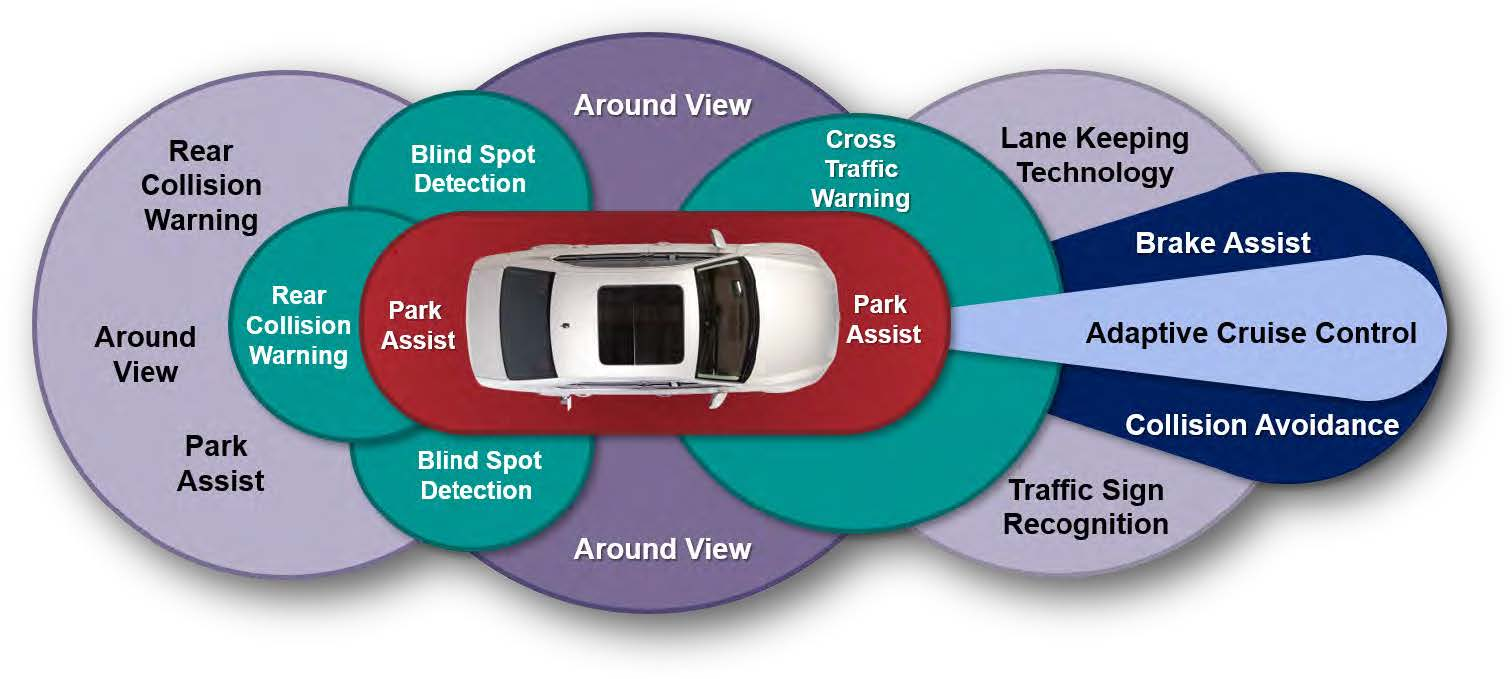
\includegraphics[width=0.6\textwidth]{Book/figures/1_introduccion/ADAS_tech.png}
    \caption{Sistema avanzado de asistencia a la conducción.}
    \label{fig:Sistema avanzado de asistencia a la conducción.}
\end{figure}

Los vehículos completamente autónomos son sistemas extremadamente complejos, por lo que actualmente no se dispone de ninguno enteramente autónomo. Por ello, mientras se avanza en el desarrollo e investigación de sistemas \ac{ADS}, son los sistemas de ayuda a la conducción o \ac{ADAS}, aquellos con los que nos podemos encontrar hoy en día. En este tipo de tecnologías es donde se centra la regulación vigente, ya que son tecnologías más probadas y que forman parte de los sistemas completamente autónomos a los que se quiere llegar. El caso de la Unión Europea muestra la evolución de la industria automovilística hacia la automatización de los sistemas de conducción, ya que a partir de julio de 2022 será obligatorio por ley el uso de tecnologías como: los sistemas de centrado en el carril, el frenado automático en caso de colisión o el uso de un sistema \ac{ISA} para regular la velocidad de los vehículos a la indicada en las vías. Todo ello para permitir obtener un mayor grado de seguridad al volante al añadir mejoras tales como las que se observan en la Figura \ref{fig:Sistema avanzado de asistencia a la conducción.}, que repercuten directamente sobre los usuarios de los vehículos \cite{adas_spain, adas_eu}.

Debido al desarrollo paulatino de estos sistemas de conducción autónoma, la \ac{SAE} ha definido 6 niveles de automatización que van del 0 (totalmente manual) al 5 (totalmente autónomo) \cite{autonomy_levels}. Estos niveles han sido adoptados por el Departamento de Transporte de los Estados Unidos, por lo que siendo un estándar actual para la clasificación de vehículos inteligentes se procede a presentar cada uno de estos niveles:

\begin{itemize}
    \item Nivel 0: La mayoría de vehículos que encontramos hoy en día en las carreteras pertenecen a este grupo, ya que con aquellos vehículos controlados manualmente.
    \item Nivel 1: Este es el nivel más bajo de automatización, ya que el vehículo cuenta únicamente con un único sistema automatizado como la dirección o la aceleración.
    \item Nivel 2: El vehículo es capaz de controlar tanto la dirección como la aceleración, pero no es un sistema autónomo ya que el conductor puede tomar el control del vehículo en cualquier momento. En esta categoría se incluyen la mayoría de los nuevos vehículos inteligentes en el mercado debido a la legislación vigente.
    \item Nivel 3: Esta clasificación se obtiene tras un gran salto tecnológico, pero para el conductor es un cambio muy sutil ya que el vehículo comienza a tener capacidades de detección del entorno lo cual permite por ejemplo, la aceleración automática del vehículo para el adelantamiento de un vehículo lento.
    \item Nivel 4: Estos vehículos son totalmente autónomos en la gran mayoría de casos, pero un conductor humano podría intervenir en una situación de emergencia. Además este tipo de vehículos suelen estar limitados en zonas urbanas a bajas velocidades.
    \item Nivel 5: Los vehículos de nivel 5 no requieren de atención humana, por lo que no será necesaria la incorporación de volante o pedales debido a su completa automatización.
\end{itemize}

\begin{figure}[H]
\centering
    \begin{subfigure}{0.45\textwidth}
    \centering
    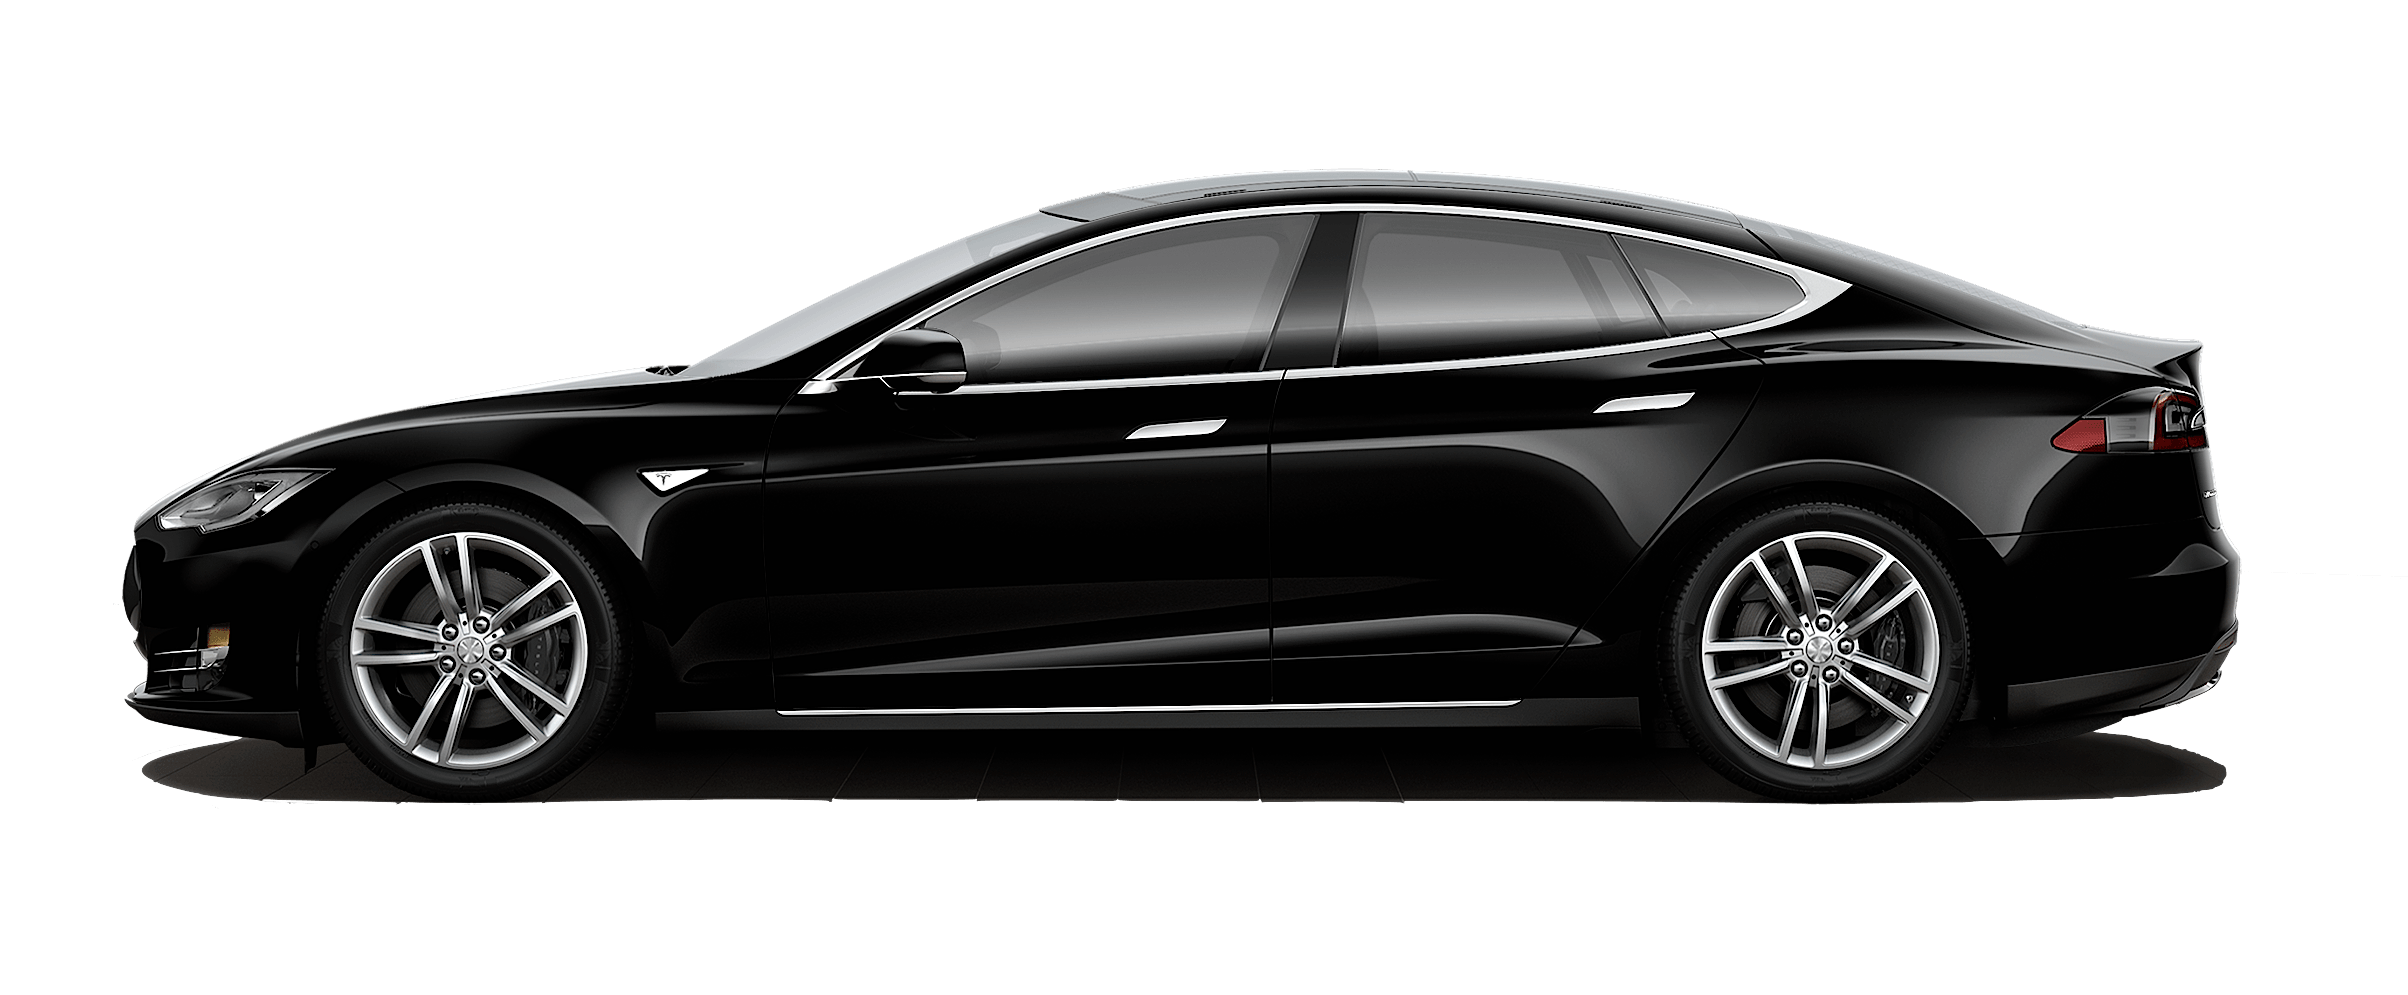
\includegraphics[width=0.95\textwidth]{Book/figures/1_introduccion/tesla.png} 
    \caption{Vehículo de Tesla.}
    \label{fig:Vehículo de Tesla.}
    \end{subfigure}
    \begin{subfigure}{0.45\textwidth}
    \centering
    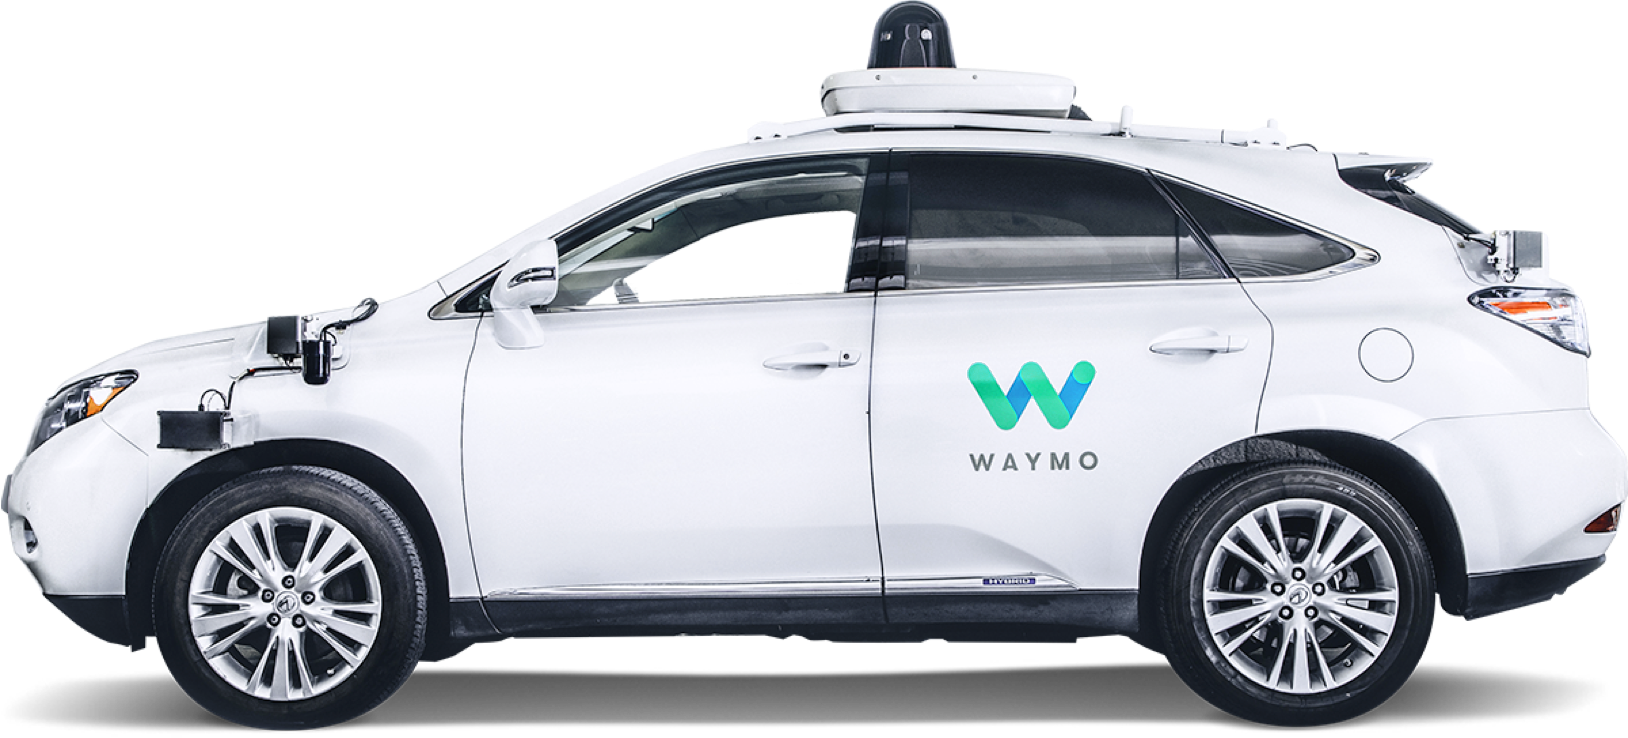
\includegraphics[width=0.85\textwidth]{Book/figures/1_introduccion/waymo.png}
    \caption{Vehículo de Waymo.}
    \label{fig:Vehículo de Waymo.}
    \end{subfigure}
\caption{Vehículos autónomos más avanzados comercializados actualmente.}
\label{fig:Vehículos autónomos más avanzados comercializados actualmente}
\end{figure}

Mientras que muchas empresas se encuentran realizando millonarias inversiones en el campo de la conducción autónoma para conseguir vehículos con la clasificación de nivel 5, entre todas ellas destaca sobre el publico general la compañía norteamericana Tesla. Pero esta no es la única empresa que está ganando mucha fama en este campo, sino que la compañía Waymo, antiguo proyecto de vehículo autónoma de Google, se encuentra entre los proyectos de creación de un vehículo de conducción autónoma completa más avanzados. Mientras que Tesla lleva años anunciando su sistema de conducción autónoma, no es hasta principios de 2022 cuando Tesla ha comenzado a mostrar la versión beta de su sistema de conducción autónoma de nivel 4. Por otra parte, Waymo se centra actualmente en la creación de una flota de taxis autónomos, este sistema se encuentra de manera funcional en Estados Unidos, en las ciudades de Phoenix y San Francisco \cite{tesla_waymo}.

Los vehículos autónomos de estas empresas no solo se diferencian en el uso actual para el cual se están comercializando, sino que como se puede observar en la Figura \ref{fig:Vehículos autónomos más avanzados comercializados actualmente}, ambos vehículos utilizan diferentes sensores para observar el entorno que les rodea. Mientras que Tesla opta por una aproximación más barata utilizando cámara y \ac{Radar}, Waymo añade al menos en la parte superior de sus vehículos un \ac{LiDAR} para la conseguir un sistema más robusto, aunque menos económico. Por lo que el desarrollo de este tipo de tecnologías puede optar por múltiples aproximaciones o configuraciones pero teniendo siempre en mente la consecución de un sistema completamente autónomo de nivel 5.

\section{Sistemas de detección de objetos}
\label{sec:Sistemas de detección de objetos}

Una de las principales tareas que realizan los vehículos autónomos es la detección de objetos, el cual se suele realizar de forma previa al seguimiento de objetos, la estimación de la trayectoria y la evitación de colisiones. Los objetos a atender en la carretera, como son: peatones, ciclistas, coches; lo cual supone un reto mayor para la creación de sistemas fiables y robustos para la detección de objetos. La mayoría de los vehículos autónomos disponibles en el mercado, así como la investigación sobre ellos, dependen del empleo de sensores costosos \cite{paper_object_detection}.

\begin{figure}[H]
    \centering
    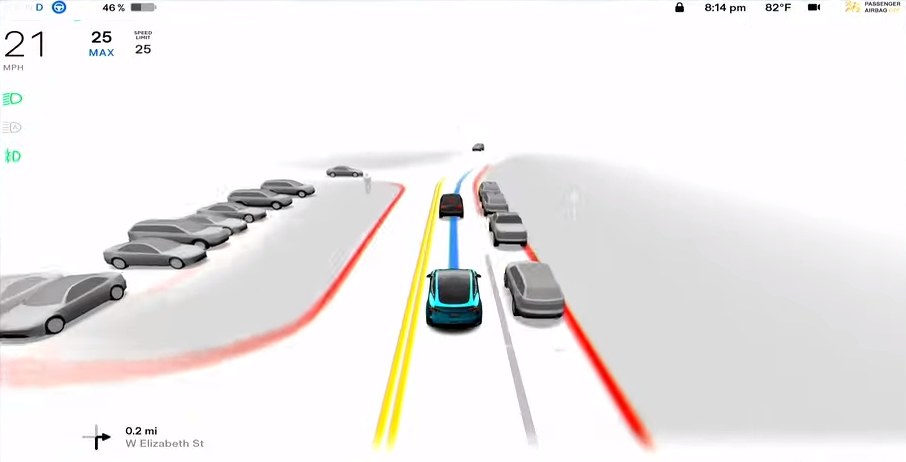
\includegraphics[width=0.65\textwidth]{Book/figures/1_introduccion/HMI_Tesla.png}
    \caption{Interfaz Humano Máquina de la beta del Tesla FDS.}
    \label{fig:Interfaz Humano Máquina de la beta del Tesla FDS.}
\end{figure}

Atendiendo a los diferentes sistemas de detección con los que se puede trabajar, encontramos los sistemas de detección 2D y detección 3D. Mientras que los sistemas de detección 2D llevan a cabo una detección de los objetos del entorno sobre el plano de las imágenes dadas por las cámaras del vehículo. Los sistemas de detección 3D pueden hacer uso de diferentes sensores para mejorar la comprensión del entorno que rodea al propio vehículo al añadir una nueva dimensión que define la profundidad, la Figura \ref{fig:Interfaz Humano Máquina de la beta del Tesla FDS.} muestra la capacidad de percepción 3D en los vehículos Tesla. Los métodos de detección 3D no solo se basan en cámaras sino que también son utilizados \ac{LiDAR} y \ac{Radar} para conseguir un sistema más preciso, ya que estos sensores se pueden utilizar tanto de forma individualizada como en conjunto para obtener un sistema de detección más robusto.

Debido a la variedad de aproximaciones que se pueden tomar en cuanto al uso de sensores para obtener un sistema de detección de objetos 3D, se procede a presentar los principales sensores utilizados tanto en la industria automovilística como en este trabajo.

\subsection{Cámara}
\label{sec:Cámara}

Los sistemas basados en cámara son los más utilizados tanto en sistemas \ac{ADAS} como sistemas \ac{ADS}, ya que permiten de forma pasiva obtener imágenes de forma continua del entorno que rodea al vehículo. Los sistemas basados en cámara tienen diferentes variaciones que se pueden utilizar, entre ellas encontramos los sistemas monoculares y los estereoscópicos. Mientras que los sistemas de cámara monoculares hacen uso de una única cámara, los sistemas de cámaras estéreo utilizan dos cámaras individuales para lograr extraer la información de profundidad de la escena a partir de técnicas como la fotogrametría, obteniendo resultados como los visibles en la Figura \ref{fig:Mapa de profundidad creado a partir de un sistema estéreo.}.

\begin{figure}[H]
    \centering
    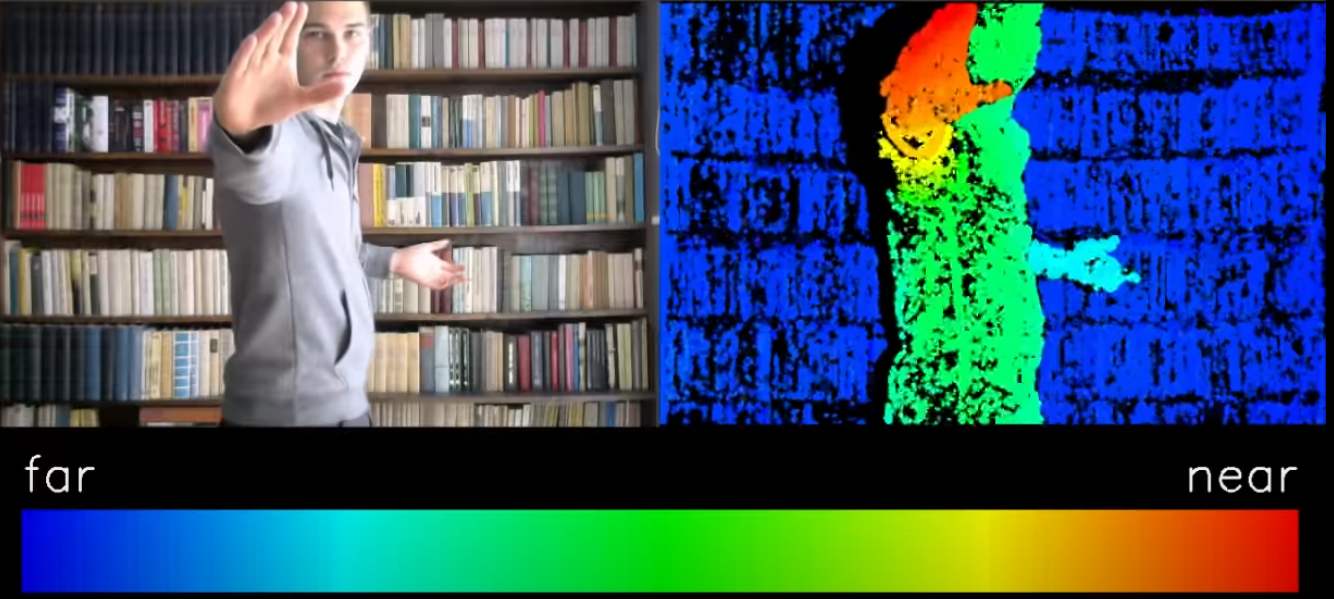
\includegraphics[width=0.65\textwidth]{Book/figures/1_introduccion/stereo_system.png}
    \caption{Mapa de profundidad creado a partir de un sistema estéreo.}
    \label{fig:Mapa de profundidad creado a partir de un sistema estéreo.}
\end{figure}

% \begin{figure}[H]
% \centering
%     \begin{subfigure}{0.45\textwidth}
%     \centering
%     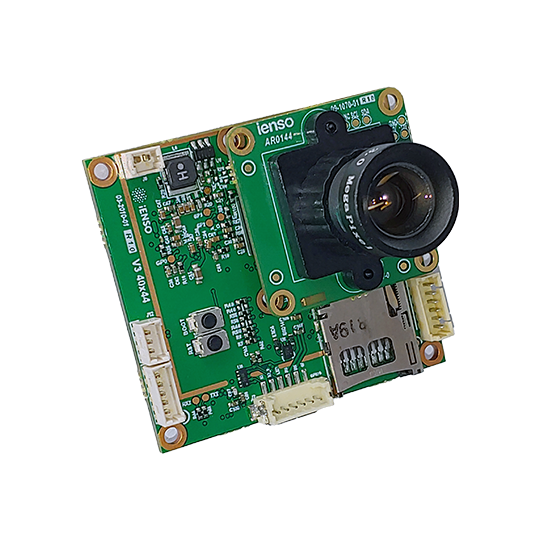
\includegraphics[width=0.5\textwidth]{Book/figures/1_introduccion/monocular_camera.png} 
%     \caption{Sistema monocular.}
%     \label{fig:Sistema monocular.}
%     \end{subfigure}
%     \begin{subfigure}{0.45\textwidth}
%     \centering
%     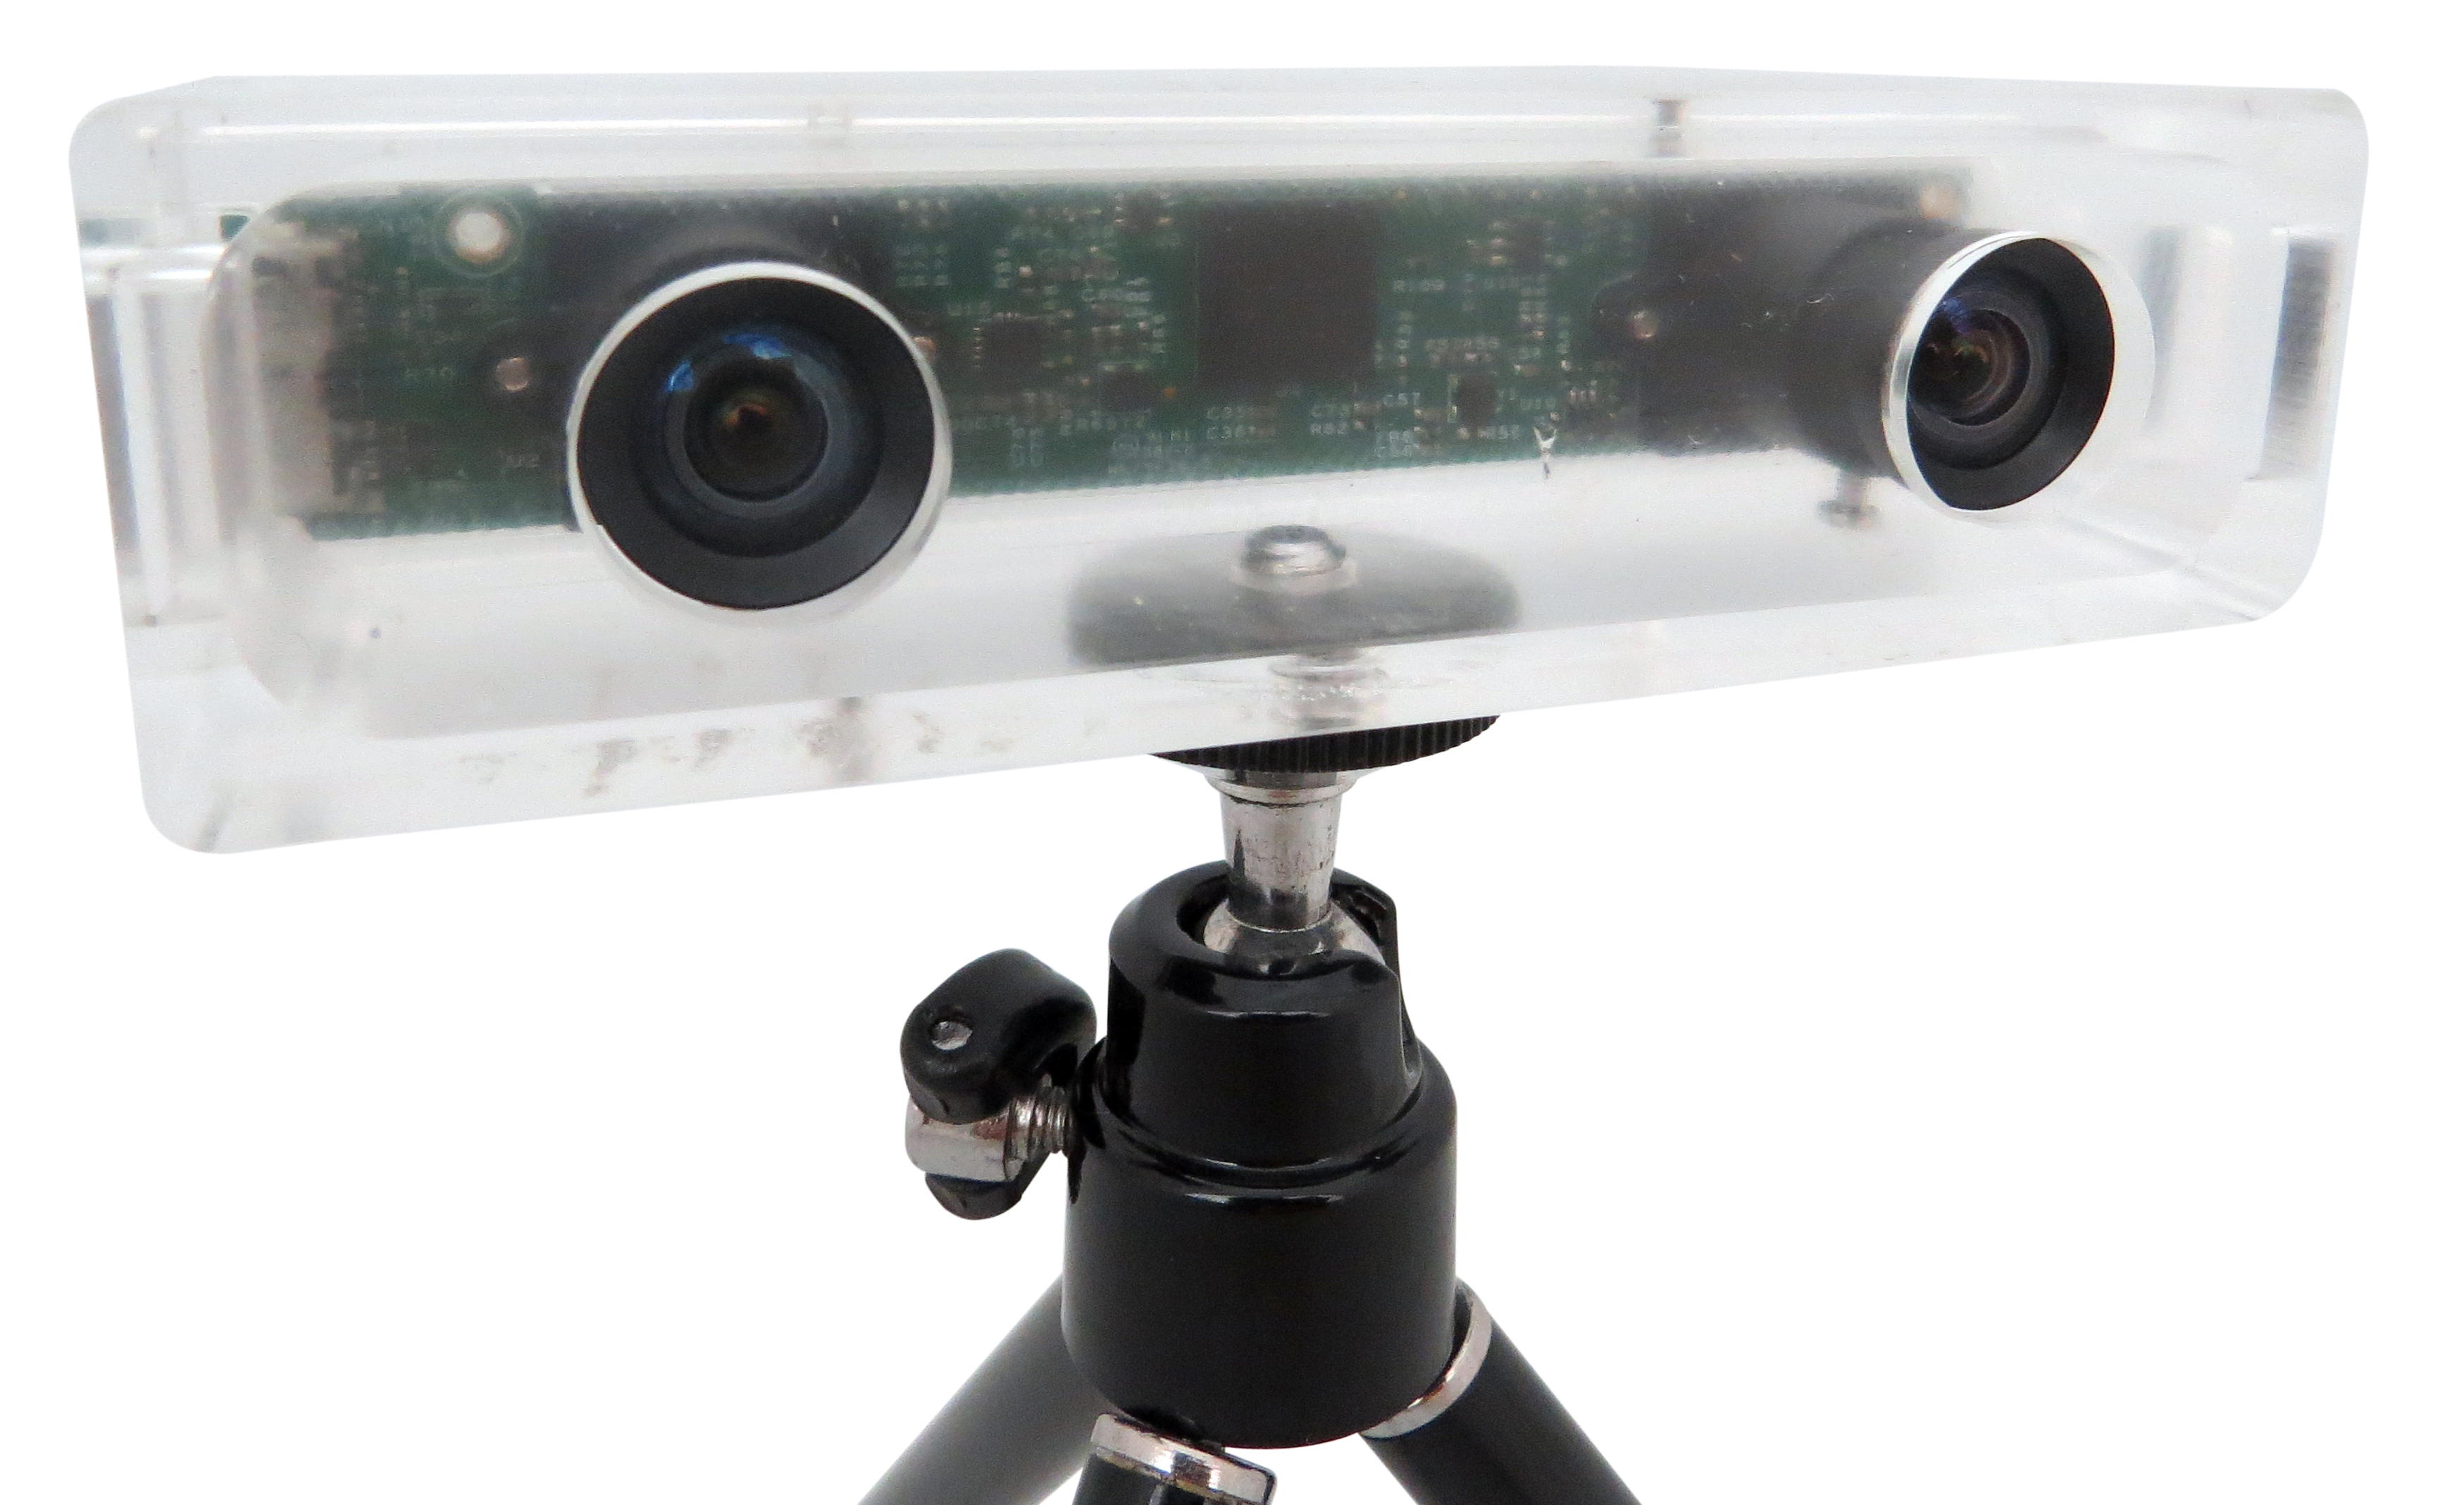
\includegraphics[width=0.85\textwidth]{Book/figures/1_introduccion/stereo_camera.png}
%     \caption{Sistema estéreo.}
%     \label{fig:Sistema estéreo.}
%     \end{subfigure}
% \caption{Diferentes sistemas de cámaras utilizados.}
% \label{fig:Diferentes sistemas de cámaras utilizados.}
% \end{figure}

Hay empresas como Tesla que basan gran parte de su sistema de conducción autónomo alrededor del uso de cámaras, debido a las ventajas que ofrece este sensor. Las cámaras son capaces de capturar la información de color, textura y contraste de forma directa, y además debido al gran estudio de técnicas basadas en Deep Learning durante los últimos años para obtener la mayor cantidad de información posible, es muy sencilla la obtención de detalles de alto nivel. Todas estas características, combinadas con gran resolución de píxeles y un bajo coste, han convertido a las cámaras en el principal candidato para los sistemas \ac{ADAS} \cite{advantages_camera}.

El uso de este sensor no se encuentra sin inconvenientes, ya que en condiciones climáticas adversas como niebla o lluvia se pierde gran parte de la información recabada por el sensor. De la misma manera que el ojo humano, las cámaras sufren con grandes cambios en la luminosidad del entorno, ya que se pueden dejar regiones sin visibilidad ninguna, como ocurre en túneles, al dirigir la cámara hacia el Sol o al conducir de noche en zonas muy oscuras. La obtención de la profundidad utilizando sistemas de cámaras requiere de un proceso muy complejo y que puede derivar en grandes errores. Por último, y como desventaja siempre presente se encuentra la necesidad de modelos basados en Deep Learning que típicamente requiere del uso de plataformas de aceleración por hardware para su uso en tiempo real \cite{paper_comparison_lidar_camera}.

\subsection{LiDAR}
\label{sec:LiDAR}

La tecnología \ac{LiDAR} se basa en la detección de los haces de luz que son emitidos por un haz de luz láser con una intensidad definida de antemano, y mide el tiempo de llegada del haz reflejado detectado por los fotodiodos que se encuentran en el sensor \cite{paper_comparison_lidar_camera, what_lidar}. Este proceso de cálculo del tiempo de llegada de cada haz láser enviado, produce una nube de puntos la cual genera un punto $(x, y, z, i)$, por cada uno de los haces de luz enviados, ya que conociendo la velocidad de la luz, el tiempo de retorno de cada haz y el ángulo de inclinación desde el que se envió, se obtiene la posición tridimensional, además del coeficiente de reflexión del objeto sobre el que el ha incidido cada rayo.

No todos los \ac{LiDAR} son iguales, ya que encontramos tanto sensores fijos que producen una nube de puntos de la parte frontal al sensor, como los encontrados en los nuevos iPhone Pro; sensores que producen una nube de puntos bidimensional al tener una plataforma giratoria con un único láser, como los utilizados en robótica móvil; y sensores con múltiples láser posicionados de forma vertical de modo que el girar mediante una plataforma giratoria producen una nube de puntos 3D, este tipo de \ac{LiDAR} es el que principalmente se utiliza para el diseño de vehículos autónomo, un ejemplo de la salida de este tipo sensores es la nube de puntos que se muestra en la Figura \ref{fig:Nube de puntos producida por un LiDAR 3D.}.

\begin{figure}[H]
    \centering
    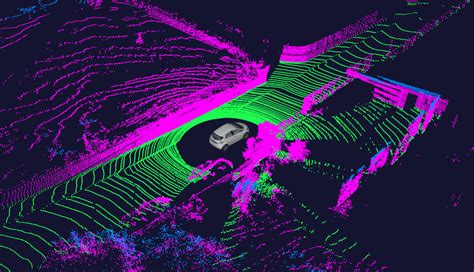
\includegraphics[width=0.6\textwidth]{Book/figures/1_introduccion/pointcloud.png}
    \caption{Nube de puntos producida por un LiDAR 3D.}
    \label{fig:Nube de puntos producida por un LiDAR 3D.}
\end{figure}

Entre las ventajas que se obtienen al utilizar un sensor \ac{LiDAR} en relación a una cámara encontramos: la precisión en las medidas tomadas, ya que el propio sensor tiene un grado de error muy reducido; el uso de los datos del \acs{LiDAR} para la obtención de la profundidad no requiere de un procesamiento previo, por lo que se puede utilizar este dato directamente recibido del sensor; las condiciones lumínicas y meteorológicas adversas no repercuten en la posibilidad de uso de dicho sensor, ya que aunque se disminuye la calidad de los datos en situaciones muy adversas, es completamente utilizable.

Al contrario, se encuentran ciertas desventajas en su uso, como la dificultad de interpretabilidad de este sensor, las condiciones climáticas en las que la obtención de datos no es perfecta y el más influyente de todos, el alto precio de este sensor que puede ascender a 100.000 dolares por un único sensor. Debido al factor monetario, este sensor no es utilizado en los vehículos de la marca Tesla ya que aumentaría considerablemente el precio de sus vehículos, aunque la gran mayoría de empresas que tratan de construir un sistema autónomo apuestan por este sensor como parte de su sistema de percepción.

\subsection{Fusión sensorial}
\label{sec:Fusión sensorial}

El uso de sensores individuales puede proporcionar información útiles del entorno que se quiere comprender. Por esto mismo, la combinación de sensores para la obtención de un sistema de percepción más preciso es un proceso que nos permite generar modelos de percepción más robustos y con menos fallos. Esto nos permite diseñar un modelo mucho mejor del mundo que nos rodea, suponiendo que el todo es mayor que la suma de sus partes. La fusión de sensores es el proceso mediante el cual podemos lograr unificar las bondades de los sensores utilizados tratando de minimizar las desventajas de cada uno de ellos \cite{what_fusion}.

Al realizar un proceso de fusión sensorial se presentan múltiples aproximaciones sobre las cuales se puede trabajar: si se realizar una unión de la información de las diferentes fuentes o en este caso sensores para construir un modelo que tome como entrada ese conjunto de datos, se trata de una 'early fusion', en cambio, si se realiza un procesamiento por cada una de las fuentes de datos y se terminan uniendo las salidas de los diferentes modelos, se obtiene un modelo basado en una 'late fusion'. Estas no son las únicas opciones disponibles, ya que entre ambas técnicas se encuentran los modelos basados en 'middle fusion' estos modelos utilizan las fuentes de datos parcialmente procesadas para unirlas y posteriormente completar el pipeline de dicho modelo, como se ve en la Figura \ref{fig:Flujo de trabajo basado en fusión sensorial.}.

\begin{figure}[H]
    \centering
    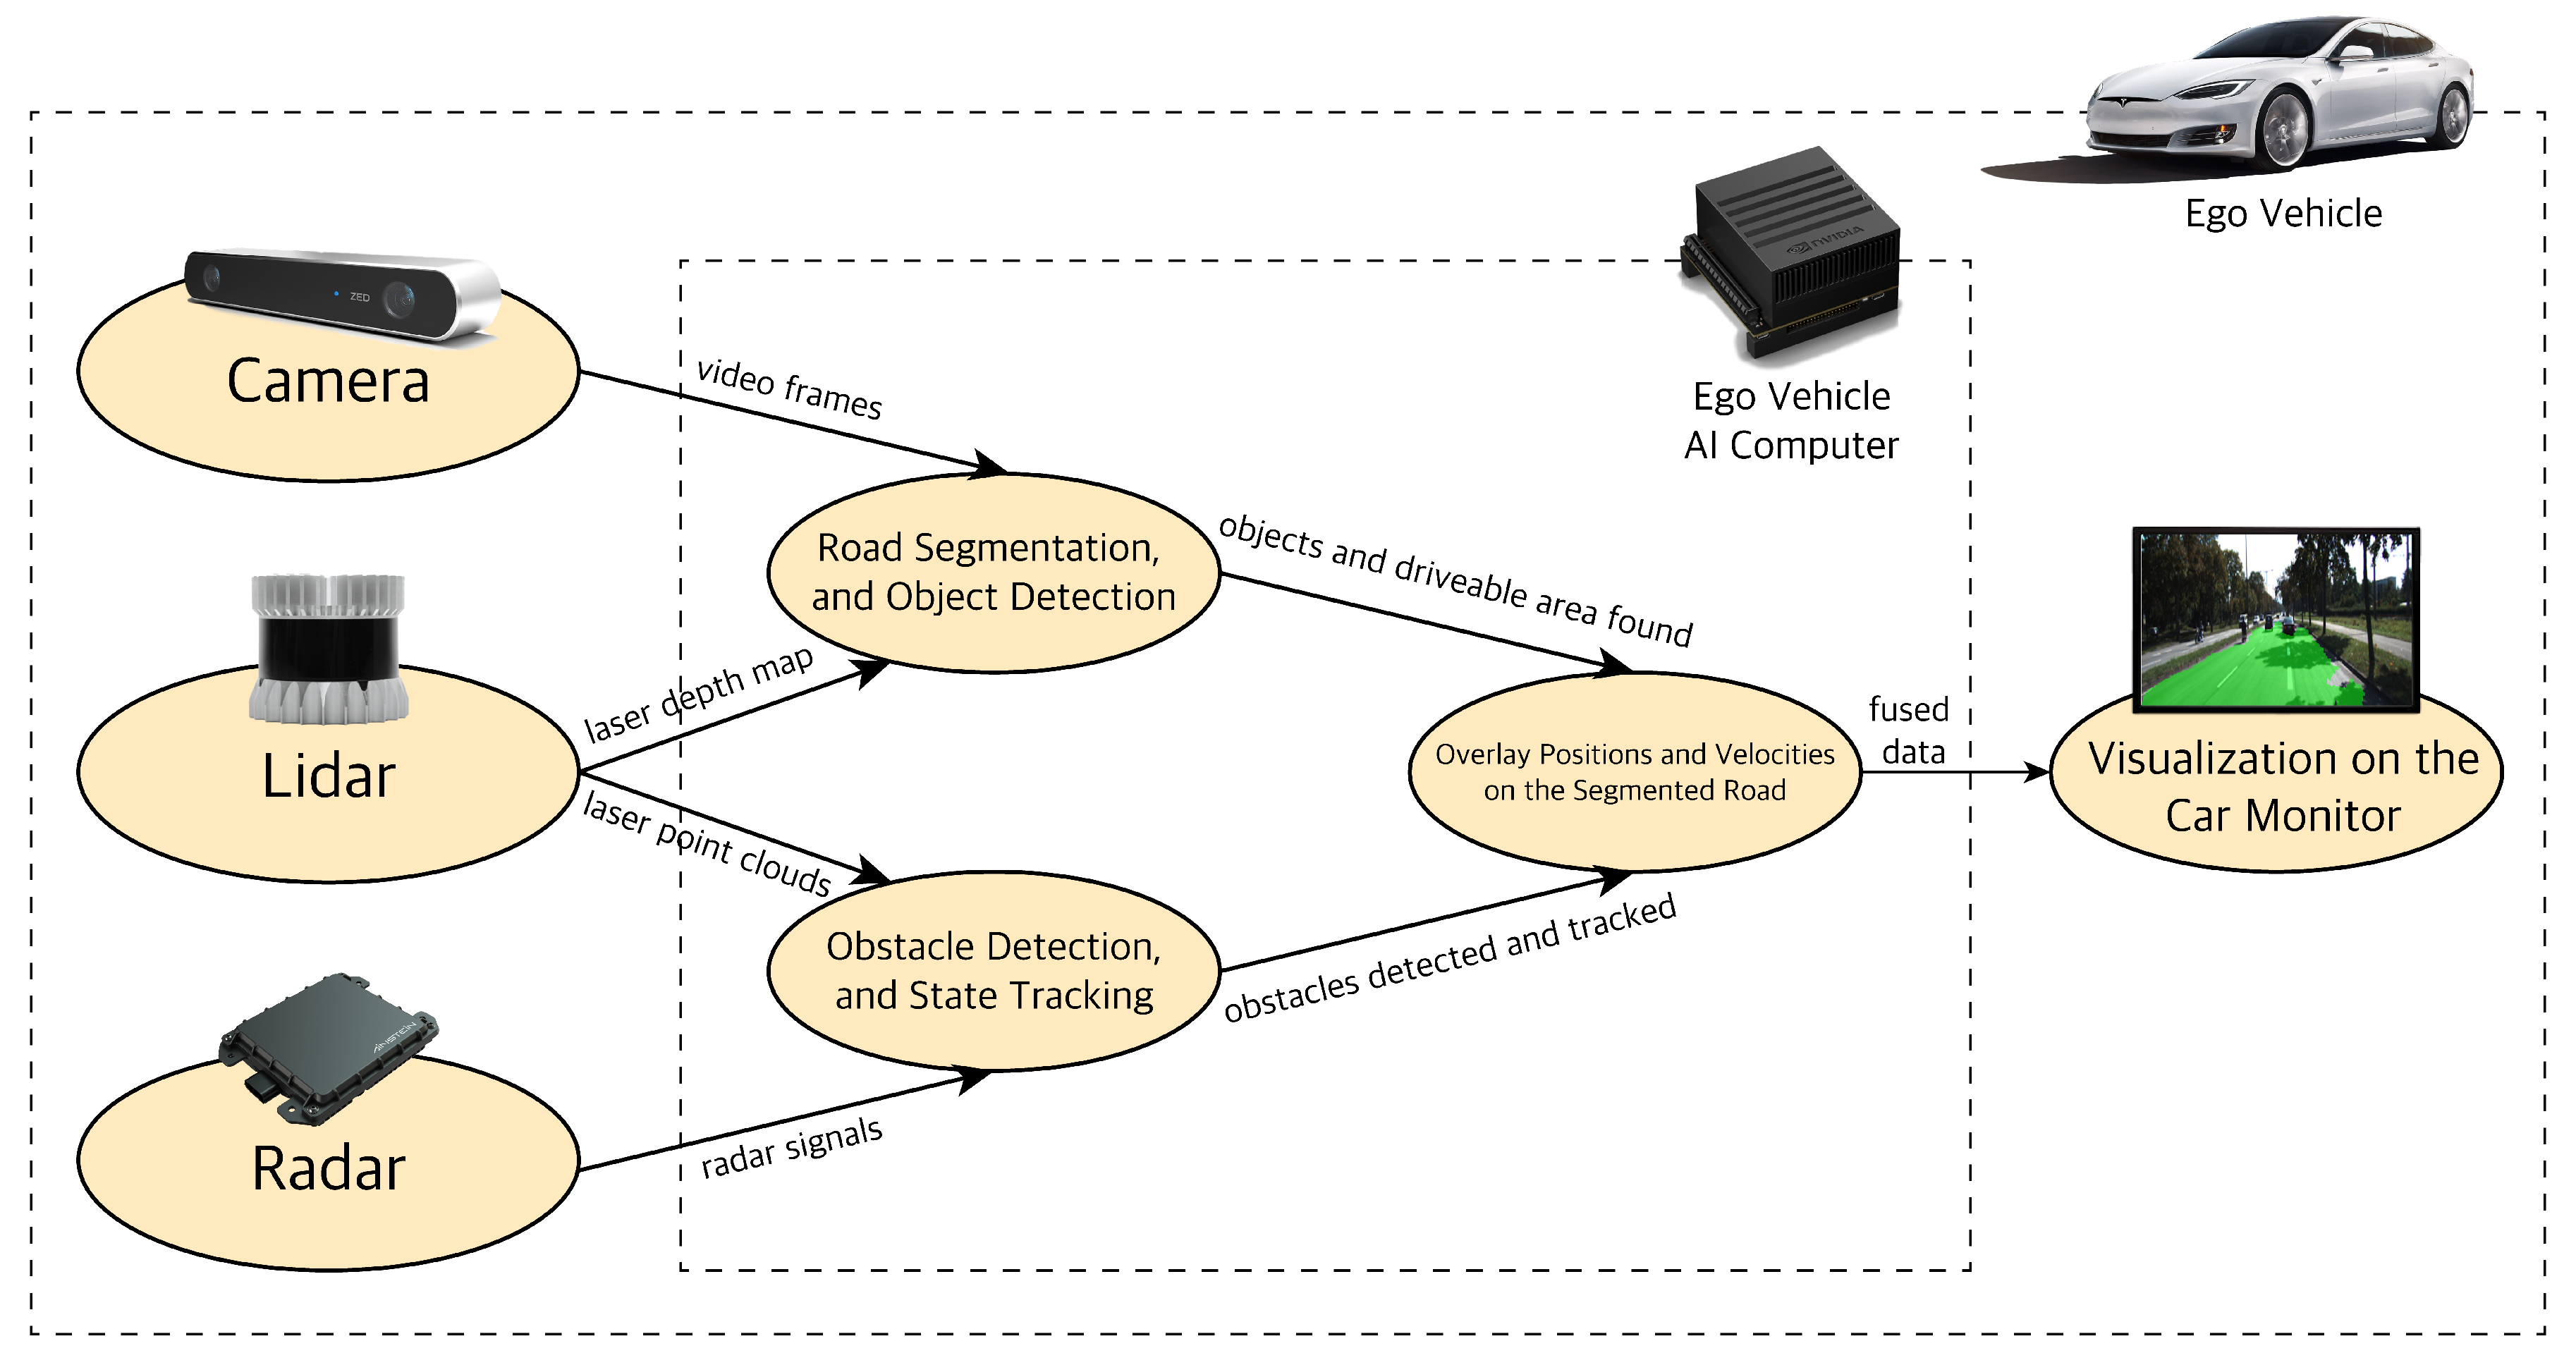
\includegraphics[width=0.7\textwidth]{Book/figures/1_introduccion/ejemplo_fusion.png}
    \caption{Flujo de trabajo basado en fusión sensorial.}
    \label{fig:Flujo de trabajo basado en fusión sensorial.}
\end{figure}

La creación de modelos de percepción basados en fusión sensorial aporta grandes ventajas sobre el uso de un único sensor, ya que permite generar sistemas más precisos y robustos al tratar de reducir las desventajas individuales de cada sensor. Entre las desventajas del uso de estos sistemas se encuentra, la complejidad en la creación del sistema completo de percepción al utilizar diferentes sensores y tecnologías, pero sobre todo el elevado coste que supone la adquisición de múltiples sensores por cada sistema de percepción. Siendo típicamente el coste, el factor vital para la producción a gran escala, la gran mayoría de las empresas basadas en la creación de sistemas de conducción autónomos abogan por el uso de esta tecnología, principalmente utilizando cámara, \ac{LiDAR} y \ac{Radar} entre otros sensores.

\section{Machine Learning}
\label{sec:Machine Learning}

El aprendizaje automático o \ac{ML} es una rama de la inteligencia artificial y la computación que se centra en el uso de datos y algoritmos para mejorar gradualmente su precisión. Mediante el uso de métodos estadísticos, los algoritmos se entrenan para hacer clasificaciones o predicciones, descubriendo ideas clave dentro de proyectos aplicando técnicas de minería de datos \cite{what_ml}.

Dentro de este amplio campo de conocimiento encontramos principalmente 4 grupos de técnicas para creación de modelos de aprendizaje automático \cite{ml_techs}:

\begin{itemize}
    \item Aprendizaje supervisado: En el caso de conocer de antemano que es lo que quiere enseñar a la máquina y se parte de una gran cantidad de datos anotados, se puede conseguir generar un modelo que se ajuste para que minimice el error al realizar la tarea que se le ha encomendado.
    \item Aprendizaje no supervisado: Este conjunto de técnicas trata de descubrir patrones ocultos que relacionen diversas variables. Además no suele requerir de grandes cantidades de datos de entrada por lo que el proceso de entrenamiento es reducido.
    \item Aprendizaje semisupervisado: Los modelos semisupervisados tratan de hacer el máximo uso de unos pocos datos etiquetados y gran cantidad de datos no etiquetados para realizar una tarea concreta.
    \item Aprendizaje por refuerzo: Mediante la interacción de una máquina con un entorno en el que poder realizar determinadas acciones que pueden ser recompensadas o castigadas, es posible generar un modelo que realice la tarea que debía realizar sin presentar explícitamente el cómo.
\end{itemize}

\begin{figure}[H]
    \centering
    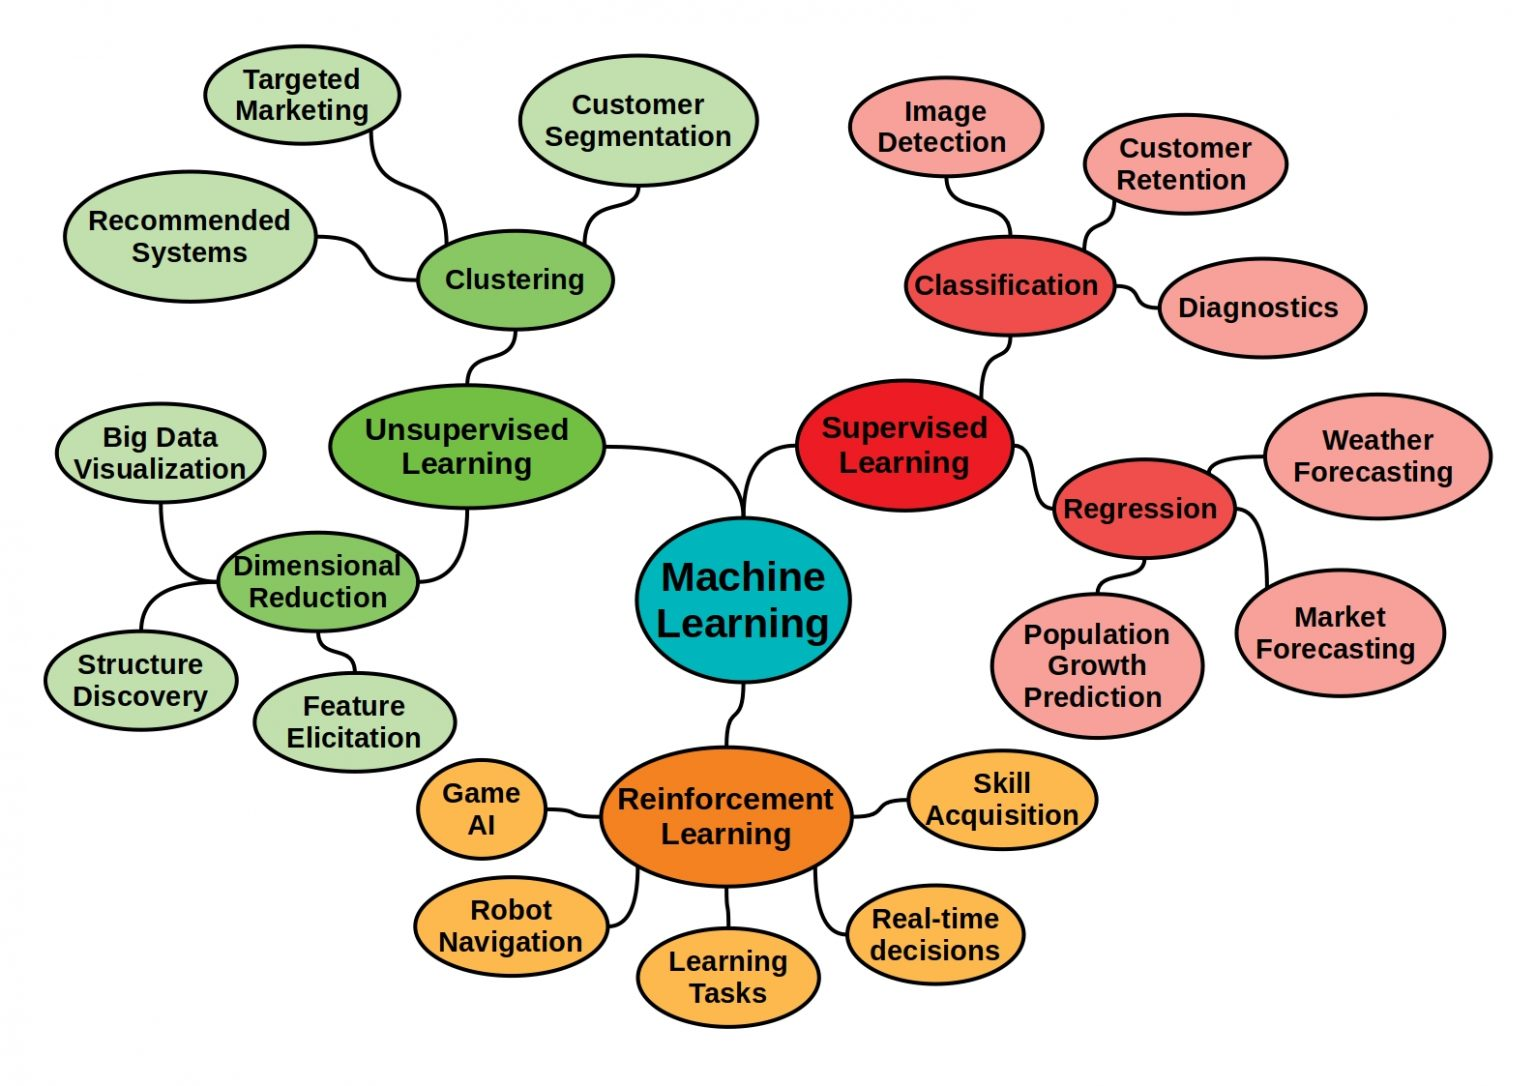
\includegraphics[width=0.6\textwidth]{Book/figures/1_introduccion/ml_techniques.png}
    \caption{Principales campos de estudio de estudio del Machine Learning.}
    \label{fig:Principales campos de estudio de estudio del Machine Learning.}
\end{figure}

A partir de estos grupos de técnicas se encuentran gran cantidad de subgrupos, como se observa en la Figura \ref{fig:Principales campos de estudio de estudio del Machine Learning.} y de técnicas concretas, pero entre todas estás técnicas, aquella que está revolucionando múltiples campos de estudio y que está propiciando grandes avances es el Deep Learning.

\subsection{Deep Learning}
\label{sec:Deep Learning}

El Deep Learning o aprendizaje profundo, es un subconjunto del campo del aprendizaje automático que consiste en el uso de redes neuronales con más una capa oculta. Dichas redes neuronales se inspiran en el cerebro humano imitando la forma en las que las neuronas biológicas se comunican entre sí. Estas se componen de una capa de nodos de entrada, una o más capas de ocultas y una capa de salida, en la que cada nodo se conecta otro y tiene un peso y umbral asociados. Si la salida de cualquier nodo individual está por encima del valor umbral especificado, ese nodo se activa, enviando datos a la siguiente capa de la red. En caso contrario, no se transmite ningún dato a la siguiente capa de la red \cite{what_nn}.

La Figura \ref{fig:Modelo básico de Deep Learning.} muestra por tanto un modelo basado en Deep Laerning ya que incorpora al menos dos capas intermedias. Mientras que una red neuronal con una sola capa puede hacer predicciones aproximadas, las capas adicionales pueden ayudar a optimizar y refinar la precisión. Los modelos basados en Deep Learning son utilizados en multitud de aplicaciones y servicios del día a día y realizan tareas analíticas y físicas sin intervención humana \cite{what_dl}. 

\begin{figure}[H]
    \centering
    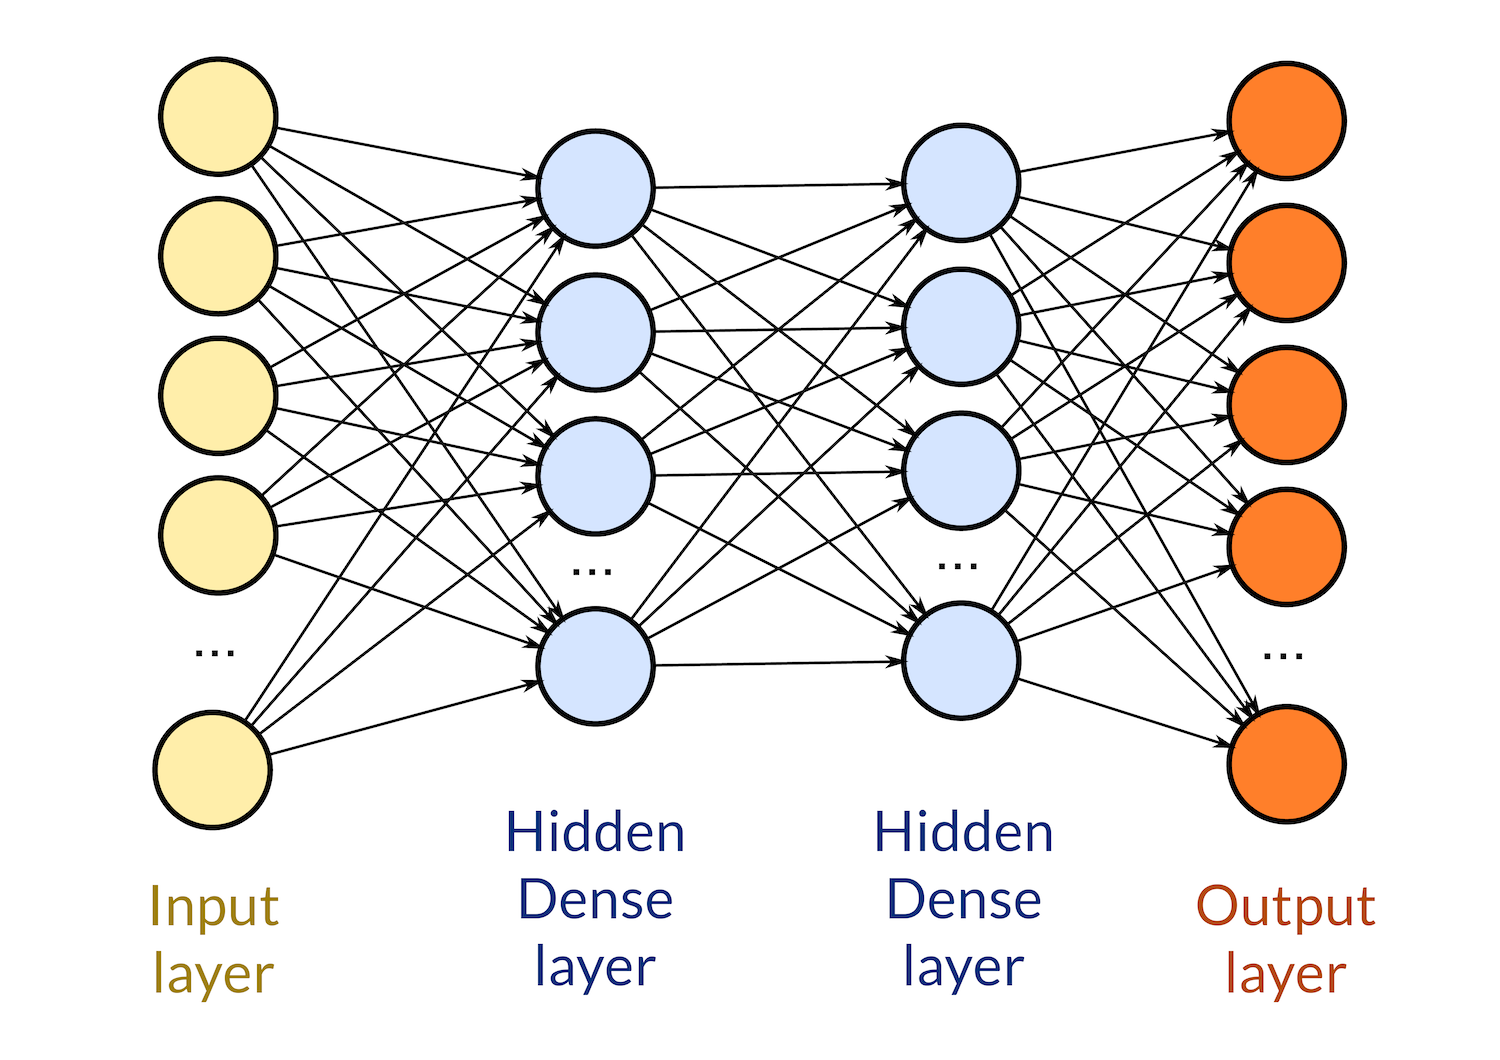
\includegraphics[width=0.6\textwidth]{Book/figures/1_introduccion/dl_model.png}
    \caption{Modelo básico de Deep Learning.}
    \label{fig:Modelo básico de Deep Learning.}
\end{figure}

Muchos campos de estudio han mejorado gracias a esta tecnología y otros están sufriendo un cambio tan radical que abren a puerta a multitud de nuevas aplicaciones que pueden ser muy beneficiosas. Entre los campos afectados por el Deep Learning encontramos:

\begin{itemize}
    \item Visión por computador: Durante los últimos años, los modelos basados en \ac{CNN} (explicados en el Capítulo \ref{sec:Convolutional Neural Networks}) han permitido el uso de sistemas de visión por computador en entornos menos controlados, ya que proporcionan una mejora espectacular en precisión en comparación con los algoritmos tradicionales de procesamiento de imágenes.
    \item Procesamiento del lenguaje natural: Tras su salida en 2020, GPT-3 \cite{GTP3} ha presentado un gran avance en el mundo del \ac{NLP} ya que ha conseguido un rendimiento inigualable hasta la fecha con grandes mejoras que vislumbran un futuro con inteligencias artificiales de carácter general.
    \item Creación de medicamentos: Dentro del campo de la medicina, hay una rama de métodos que tratan de predecir que estructura de las proteínas son las más eficaces en combatir una enfermedad. La empresa DeepMind tras la presentación del modelo basado en Deep Learning, AlphaFold \cite{AlphaFold}, y conseguir superar con amplias creces la competición \ac{CASP} que se basa en la predicción de la estructura de las proteínas, ha conseguido situarse a la cabeza de este campo democratizando a su vez el acceso a desarrollar de nuevas tecnologías a partir de esta.
\end{itemize}

Como se ha presentado, el Deep Learning engloba un conjunto de técnicas ampliamente utilizadas, esto es debido principalmente a que permite maximizar el uso de datos no estructurados, obtiene en gran cantidad de los casos unos muy buenos resultados y no requiere de una perfecta aplicación de 'feature engineering'. Como contraparte a su uso encontramos: la gran cantidad de datos que se necesitan para la creación de un modelo, la necesidad de un conocimiento especializado en las técnicas Deep Learning aplicadas al campo en el que se trabaja, y la necesidad de una gran potencia computacional para el entrenamiento de los modelos \cite{adv_disafv_dl}.
